\documentclass[journal]{IEEEtran}

% XeTeX has no Type-1 Times: load the TeX Gyre Termes (Times) files so bold and italic exist
\usepackage{fontspec}
\setmainfont{texgyretermes}[Extension=.otf, UprightFont=*-regular, BoldFont=*-bold,
  ItalicFont=*-italic, BoldItalicFont=*-bolditalic]
\setsansfont{texgyreheros}[Extension=.otf, UprightFont=*-regular, BoldFont=*-bold,
  ItalicFont=*-italic, BoldItalicFont=*-bolditalic]

\usepackage{cite}
\usepackage{amsmath,amssymb,amsfonts}
\usepackage{graphicx}
\usepackage{booktabs}
\usepackage{multirow}
\usepackage{array}
\usepackage{algorithm}
\usepackage{algpseudocode}
\usepackage{xcolor}
\usepackage{tikz}
\usetikzlibrary{arrows.meta,positioning,fit,calc}
\usepackage[hidelinks]{hyperref}

% generated by make_numbers.py from results/puformer_chikusei_x4_v3/paper_analysis/q2n.json
\newcommand{\QtwonVthree}{0.9931}
\newcommand{\QtwonExactUV}{0.9988}
\newcommand{\QtwonExactUVNIR}{0.9998}
\newcommand{\RelErrUV}{0.41}
\newcommand{\RelErrMaxOther}{0.040}
\newcommand{\OracleBicA}{61.6}
\newcommand{\OracleLinA}{57.5}
\newcommand{\OracleModelA}{51.8}
\newcommand{\DefTen}{25\%}
\newcommand{\DefFifty}{75\%}
\newcommand{\CalibPsnrHi}{58.20}
\newcommand{\CalibQHi}{0.9931}
\newcommand{\CalibPsnrMid}{52.15}
\newcommand{\CalibQMid}{0.9904}


\newcommand{\best}[1]{\textbf{#1}}
\newcommand{\bm}[1]{\boldsymbol{#1}}
\newcommand{\X}{\mathbf{X}}
\newcommand{\Z}{\mathbf{Z}}
\newcommand{\YH}{\mathbf{Y}_{\mathrm{H}}}
\newcommand{\YM}{\mathbf{Y}_{\mathrm{M}}}
\newcommand{\D}{\mathcal{D}}
\newcommand{\R}{\mathcal{R}}

\begin{document}

\title{PUFormer: A Physics-Unfolded Transformer With Exact Observation Operators for Hyperspectral and Multispectral Image Fusion}

\author{Amarnath~M%
\thanks{E-mail: amarnath10chinu@gmail.com. Code, training logs and all result files are available at
\url{https://github.com/Amarnath10i/Research-On-Hyperspectral-ImageFussion}.}}

\markboth{Preprint}{Amarnath: PUFormer for Hyperspectral and Multispectral Image Fusion}

\maketitle

\begin{abstract}
Fusing a low-resolution hyperspectral image (LR-HSI) with a high-resolution multispectral image (HR-MSI) is an ill-posed inverse problem whose forward model is usually known exactly in benchmark settings, yet most deep fusion networks either ignore the model or apply it only approximately. We present PUFormer, a physics-unfolded transformer that alternates exact data-consistency steps with a learned spectral-attention prior. Each stage takes a gradient step on both observation residuals using the true blur--decimation operator and spectral response and their exact adjoints, including the reflect-padded image border that the data simulation uses, and then corrects the result with a three-level U-Net of transposed-attention transformer blocks that carries features from one stage to the next. The network is trained with an L1 loss, deep supervision and small spectral-angle and structural-similarity terms. On the Chikusei $\times$4 benchmark with a WorldView-2 multispectral sensor, under the protocol of a recent IEEE TIP study that compared 17 methods, PUFormer reaches 58.20~dB PSNR, a spectral angle of 0.713$^\circ$, an ERGAS of 1.330 and an RMSE of 18.9 digital numbers with 10.1~M parameters, ranking first on seven of the eight reported metrics. Its reconstructions reproduce both inputs to within 86--90~dB, and when the true blur is supplied at test time the model stays within 0.26~dB of its nominal accuracy for blur widths it was not trained on. We further show that the remaining Q2n gap is dominated by ultraviolet bands that lie outside the multispectral sensor's range and whose fine detail is noise-like, and we release the code, logs and evaluation scripts.
\end{abstract}

\begin{IEEEkeywords}
Hyperspectral image fusion, multispectral image, deep unfolding, transformer, super-resolution, Chikusei.
\end{IEEEkeywords}

\section{Introduction}
\IEEEPARstart{H}{yperspectral} imagers record hundreds of narrow spectral bands but, for a fixed photon budget, at a coarse spatial resolution; multispectral imagers do the opposite. Hyperspectral and multispectral image fusion recovers a high-resolution hyperspectral image (HR-HSI) from one observation of each kind~\cite{yokoya2017review,loncan2015review,vivone2025deep}. Classical methods formulate fusion as a regularized inverse problem, using component substitution~\cite{aiazzi2007gsa}, coupled matrix factorization~\cite{yokoya2012cnmf}, subspace regularization~\cite{simoes2015hysure} or fast Sylvester-equation solvers~\cite{wei2015fuse}. Deep networks have since become the dominant approach, from convolutional reconstruction networks~\cite{zhang2021ssrnet,ran2023guidednet} to transformers~\cite{deng2023psrt,fang2024mimosst,he2024lgct,fu2025ssdt} and diffusion models~\cite{cao2024ddif,chen2026twostage,xu2026cdps,zhu2025argsdiff}.

Two observations motivate this work. First, in the simulated benchmarks on which fusion methods are ranked, the degradation from the HR-HSI to each observation is known exactly, yet most networks treat both observations as generic inputs. Model-guided and unfolded networks~\cite{xie2022mhfnet,dong2021mogdcn,fang2024dunet,tian2024hmpnet,sun2025iatun} do use the operators, but they typically apply zero-padded or approximate versions that do not match the operator that generated the data at the image border, so even the ground truth fails the network's own consistency check there. Second, reported numbers on the same dataset vary by tens of decibels across papers because of differences in the sensor response, blur, split, normalization and even the definition of each metric~\cite{vivone2025deep}. Claims of improvement are therefore only meaningful within one fully specified protocol.

We address both points on the Chikusei dataset~\cite{yokoya2016chikusei} under the protocol of Chen~\textit{et al.}~\cite{chen2026twostage} (WorldView-2 multispectral response, $7\times7$ Gaussian blur with $\sigma=2$, $\times4$ decimation, eight $256\times256$ test images), which reports 17 methods on eight metrics. Our contributions are:
\begin{enumerate}
\item \textbf{PUFormer}, a physics-unfolded network whose data-consistency steps use the exact forward operators and their exact adjoints, including the reflect-padded border of the simulation, combined with a transposed-attention U-Net prior~\cite{zamir2022restormer} that carries memory across stages.
\item A \textbf{complete and reproducible evaluation}: eight metrics implemented from their reference code, three PSNR and two SSIM definitions reported side by side, per-image results, and the consistency of each reconstruction with its own inputs.
\item \textbf{State-of-the-art accuracy} on this protocol: 58.20~dB PSNR (+2.01~dB over the best reported method), first on seven of eight metrics, with 10.1~M parameters.
\item \textbf{Robustness and failure analysis}: a test-time operator swap that almost fully compensates blur mismatch, a noise study, and an analysis showing that the Q2n shortfall comes from bands without multispectral coverage.
\end{enumerate}

\section{Related Work}
\subsection{Model-based fusion}
Component substitution methods such as GSA~\cite{aiazzi2007gsa} inject multispectral detail into the upsampled hyperspectral bands. Unmixing-based methods such as CNMF~\cite{yokoya2012cnmf} factor both observations with shared endmembers, and subspace methods such as HySure~\cite{simoes2015hysure} regularize the HR-HSI within a low-dimensional spectral subspace, whose dimension can be estimated with HySime~\cite{bioucas2008hysime}. FUSE~\cite{wei2015fuse} solves the resulting quadratic problem in closed form through a Sylvester equation. These methods use the forward model explicitly but rely on hand-crafted priors.

\subsection{Supervised deep fusion}
SSR-NET~\cite{zhang2021ssrnet} and GuidedNet~\cite{ran2023guidednet} learn a direct mapping from the two observations. Transformers model long-range spatial and spectral dependencies: PSRT~\cite{deng2023psrt} uses pyramid shuffle-and-reshuffle attention, MIMO-SST~\cite{fang2024mimosst} multi-input multi-output supervision, LGCT~\cite{he2024lgct} local--global collaboration, DSPNet~\cite{shan2023dspnet} a dual spatial--spectral pyramid, SSDT~\cite{fu2025ssdt} dilated attention, and MIMFormer~\cite{li2024mimformer}, AMSF-Net~\cite{liu2025amsf}, ASMNet~\cite{liu2025asmnet} and DPFormer~\cite{liu2026dpformer} multiscale spectral--spatial designs. Recent work also studies state-space models~\cite{peng2024fusionmamba,huang2026hdgmamba}, mixture-of-experts routing~\cite{xiao2026ramoe} and modality interaction~\cite{huo2026mian}. General image-fusion frameworks such as U2Net~\cite{peng2023u2net} and OTPNet~\cite{yu2025otpnet} have also been applied to this task.

\subsection{Model-guided and unfolded networks}
Algorithm unrolling~\cite{gregor2010lista,monga2021unrolling,zhang2018istanet} turns the iterations of an optimization method into network stages. MHF-Net~\cite{xie2022mhfnet} and MoG-DCN~\cite{dong2021mogdcn} unfold fusion-specific solvers, DUNET~\cite{fang2024dunet} adds transformer priors for unregistered inputs, HMPNet~\cite{tian2024hmpnet} extends unfolding to three modalities, and an information-aware transformer-based unfolding network~\cite{sun2025iatun} and a mutual-guidance unfolding network (SMGU)~\cite{yan2025smgu} strengthen the learned proximal steps. PUFormer belongs to this family. It differs in using the exact simulation operator at the image border, in its cross-stage memory and in its transposed-attention prior, which attends across spectral feature channels rather than spatial windows.

\subsection{Generative fusion}
Diffusion models have been conditioned on the two observations (DDIF~\cite{cao2024ddif}), constrained by the observation model during sampling (CDPS~\cite{xu2026cdps}), restricted to a learned subspace (ARGS-Diff~\cite{zhu2025argsdiff}) or combined with differential attention in a two-stage conditioning scheme~\cite{chen2026twostage}. Null-space formulations~\cite{wang2023ddnm} make the data-consistency part of the reconstruction exact. The two-stage conditional diffusion model of Chen~\textit{et al.}~\cite{chen2026twostage} holds the best published Chikusei $\times$4 results in our survey and is our main reference; its comparison also includes the correlation-aware network CLSNet~\cite{yang2026clsnet} and the dual cross transformer (DCTransformer)~\cite{ma2024reciprocal}, denoted DCT in their table.

\section{Observation Model and Exact Operators}
\label{sec:model}
Let $\X\in\mathbb{R}^{B\times H\times W}$ be the HR-HSI with $B=128$ bands. The two observations are
\begin{equation}
\YH = \D\X,\qquad \YM = \R\X,
\label{eq:obs}
\end{equation}
where $\D=\mathcal{S}\,\mathcal{K}\,\mathcal{P}$ applies, band by band, reflect padding $\mathcal{P}$ of width $p=3$, a valid correlation $\mathcal{K}$ with a normalized $7\times7$ Gaussian kernel ($\sigma=2$), and decimation $\mathcal{S}$ that keeps every fourth pixel starting at index zero, so $\YH\in\mathbb{R}^{B\times H/4\times W/4}$. The spectral operator $\R\in\mathbb{R}^{M\times B}$ integrates the spectrum with the $M=8$ WorldView-2 band responses~\cite{digitalglobe2014srf}. Because the manufacturer publishes the responses only as plots together with the 5\%-response band edges, we model each band as a flat top with logistic flanks (4~nm roll-off) that reach 5\% exactly at the tabulated edges, and normalize every band to unit sum.

\textbf{Exact adjoint.} Every gradient step on $\|\D\X-\YH\|^2$ requires $\D^{\top}=\mathcal{P}^{\top}\mathcal{K}^{\top}\mathcal{S}^{\top}$. $\mathcal{S}^{\top}$ inserts zeros and $\mathcal{K}^{\top}$ is a full convolution; together they are a strided transposed convolution with an output padding of three. The adjoint of reflect padding folds the padded margins back onto the pixels they were copied from. For a padded row index $j\in[0,H+2p)$ the source row is $p-j$ for $j<p$, $j-p$ in the interior and $2H-2+p-j$ in the bottom margin, hence
\begin{equation}
\begin{split}
(\mathcal{P}^{\top}\mathbf{g})_i={}&\mathbf{g}_{i+p}+[1\le i\le p]\,\mathbf{g}_{p-i}\\
&+[H-1-p\le i\le H-2]\,\mathbf{g}_{2H-2+p-i},
\end{split}
\label{eq:fold}
\end{equation}
applied to rows and then to columns. Most unfolded networks instead use zero padding inside the network while the data are generated with a different border rule; the ground truth then does not satisfy~\eqref{eq:obs} in the network's own operator, and the data-consistency step pushes the first rows and columns of every image in the wrong direction. With~\eqref{eq:fold}, $\D$ in the network is exactly the simulation operator, and the inner-product test $\langle\D\X,\mathbf{Y}\rangle=\langle\X,\D^{\top}\mathbf{Y}\rangle$ holds to a relative error of $10^{-16}$ in double precision. $\R^{\top}$ is the transpose of the response matrix.

\section{PUFormer}
\label{sec:method}
\begin{figure*}[t]
\centering
\resizebox{\textwidth}{!}{%
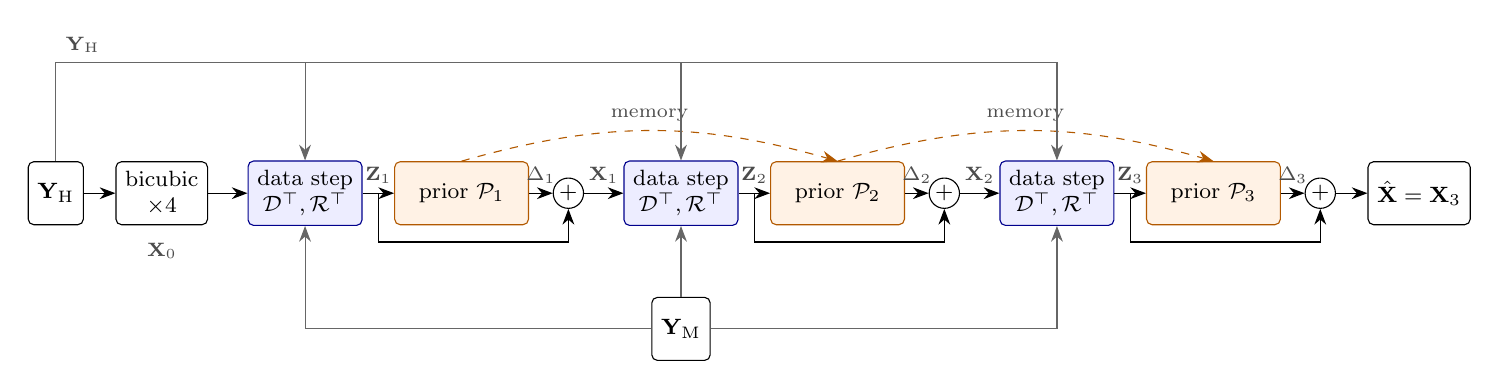
\begin{tikzpicture}[
  font=\footnotesize, >={Stealth[length=2mm]},
  box/.style={draw, rounded corners=2pt, minimum height=8mm, align=center, fill=white},
  phys/.style={box, fill=blue!7, draw=blue!55!black},
  prior/.style={box, fill=orange!10, draw=orange!70!black, minimum width=17mm},
  op/.style={circle, draw, inner sep=0.8pt},
  lab/.style={font=\scriptsize, text=black!70}]
\node[box] (yh) {$\YH$};
\node[box, right=4mm of yh] (bic) {bicubic\\$\times4$};
\node[lab, below=1mm of bic] {$\X_0$};
\node[phys, right=5mm of bic] (d1) {data step\\$\D^{\top},\R^{\top}$};
\node[prior, right=4mm of d1] (p1) {prior $\mathcal{P}_1$};
\node[op, right=3mm of p1] (a1) {$+$};
\node[phys, right=5mm of a1] (d2) {data step\\$\D^{\top},\R^{\top}$};
\node[prior, right=4mm of d2] (p2) {prior $\mathcal{P}_2$};
\node[op, right=3mm of p2] (a2) {$+$};
\node[phys, right=5mm of a2] (d3) {data step\\$\D^{\top},\R^{\top}$};
\node[prior, right=4mm of d3] (p3) {prior $\mathcal{P}_3$};
\node[op, right=3mm of p3] (a3) {$+$};
\node[box, right=4mm of a3] (out) {$\hat{\X}=\X_3$};
\node[box, below=9mm of d2] (ym) {$\YM$};
\draw[->] (yh) -- (bic); \draw[->] (bic) -- (d1);
\draw[->] (d1) -- node[above, lab]{$\Z_1$} (p1); \draw[->] (p1) -- node[above, lab]{$\Delta_1$} (a1);
\draw[->] (a1) -- node[above, lab]{$\X_1$} (d2);
\draw[->] (d2) -- node[above, lab]{$\Z_2$} (p2); \draw[->] (p2) -- node[above, lab]{$\Delta_2$} (a2);
\draw[->] (a2) -- node[above, lab]{$\X_2$} (d3);
\draw[->] (d3) -- node[above, lab]{$\Z_3$} (p3); \draw[->] (p3) -- node[above, lab]{$\Delta_3$} (a3);
\draw[->] (a3) -- (out);
\draw[->] ($(d1.east)!0.5!(p1.west)$) |- ++(0,-0.62) -| (a1.south);
\draw[->] ($(d2.east)!0.5!(p2.west)$) |- ++(0,-0.62) -| (a2.south);
\draw[->] ($(d3.east)!0.5!(p3.west)$) |- ++(0,-0.62) -| (a3.south);
\draw[->, dashed, orange!70!black] (p1.north) to[bend left=16] node[above, lab]{memory} (p2.north);
\draw[->, dashed, orange!70!black] (p2.north) to[bend left=16] node[above, lab]{memory} (p3.north);
\draw[->, black!60] (ym) -| (d1.south); \draw[->, black!60] (ym) -- (d2.south); \draw[->, black!60] (ym) -| (d3.south);
\coordinate (bus) at ($(yh.north)+(0,1.25)$);
\draw[->, black!60] (yh.north) -- (bus) -| (d3.north);
\draw[->, black!60] (d1.north |- bus) -- (d1.north);
\draw[->, black!60] (d2.north |- bus) -- (d2.north);
\node[lab, above right] at (bus) {$\YH$};
\end{tikzpicture}}
\vspace{1mm}

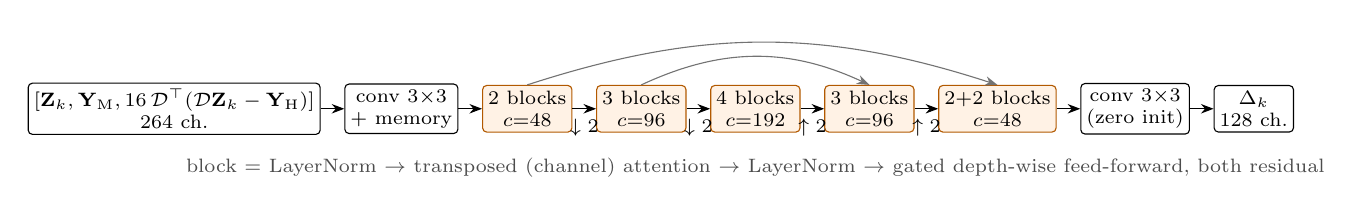
\begin{tikzpicture}[font=\scriptsize, >={Stealth[length=1.6mm]},
  blk/.style={draw, rounded corners=1.5pt, fill=orange!10, draw=orange!70!black, minimum height=5.5mm, align=center, inner sep=2pt},
  pl/.style={draw, rounded corners=1.5pt, fill=white, minimum height=5.5mm, align=center, inner sep=2pt}]
\node[pl] (in) {$[\Z_k,\YM,16\,\D^{\top}(\D\Z_k-\YH)]$\\264 ch.};
\node[pl, right=3mm of in] (emb) {conv $3{\times}3$\\+ memory};
\node[blk, right=3mm of emb] (e1) {2 blocks\\$c{=}48$};
\node[blk, right=3mm of e1] (e2) {3 blocks\\$c{=}96$};
\node[blk, right=3mm of e2] (m) {4 blocks\\$c{=}192$};
\node[blk, right=3mm of m] (d2) {3 blocks\\$c{=}96$};
\node[blk, right=3mm of d2] (d1) {2+2 blocks\\$c{=}48$};
\node[pl, right=3mm of d1] (tail) {conv $3{\times}3$\\(zero init)};
\node[pl, right=3mm of tail] (res) {$\Delta_k$\\128 ch.};
\draw[->] (in)--(emb); \draw[->] (emb)--(e1); \draw[->] (e1)--node[below]{$\downarrow2$}(e2); \draw[->] (e2)--node[below]{$\downarrow2$}(m);
\draw[->] (m)--node[below]{$\uparrow2$}(d2); \draw[->] (d2)--node[below]{$\uparrow2$}(d1); \draw[->] (d1)--(tail); \draw[->] (tail)--(res);
\draw[->, black!55] (e2.north) to[bend left=25] (d2.north);
\draw[->, black!55] (e1.north) to[bend left=18] (d1.north);
\node[below=2mm of m, align=center, text=black!70] {block $=$ LayerNorm $\to$ transposed (channel) attention $\to$ LayerNorm $\to$ gated depth-wise feed-forward, both residual};
\end{tikzpicture}
\caption{PUFormer. Top: three unfolded stages, each an exact data-consistency step on both observations followed by a learned residual prior; decoder features are passed to the next stage's prior (memory). Bottom: the prior of stage $k$, a three-level U-Net of transposed-attention transformer blocks.}
\label{fig:arch}
\end{figure*}

\subsection{Unfolded iterations}
PUFormer (Fig.~\ref{fig:arch}) starts from the bicubic upsampling $\X_0$ of $\YH$ and performs $K=3$ stages. Stage $k$ first takes a gradient step on both data terms,
\begin{equation}
\begin{split}
\Z_k=\X_{k-1}&-16\,\alpha_k\,\D^{\top}(\D\X_{k-1}-\YH)\\
&-\beta_k\,\R^{\top}(\R\X_{k-1}-\YM),
\end{split}
\label{eq:step}
\end{equation}
with learnable step sizes $\alpha_k=\mathrm{softplus}(a_k)$ and $\beta_k=\mathrm{softplus}(b_k)$. The factor 16 compensates the $1/16$ gain of $\D^{\top}\D$ on smooth content under $\times4$ decimation, so that both steps start at a comparable scale. The prior then predicts a residual,
\begin{equation}
\begin{split}
(\Delta_k,\mathbf{F}_k)&=\mathcal{P}_k\big([\Z_k,\YM,16\,\D^{\top}(\D\Z_k-\YH)],\,\mathbf{F}_{k-1}\big),\\
\X_k&=\Z_k+\Delta_k,
\end{split}
\label{eq:prior}
\end{equation}
where the third input tells the prior where the updated estimate still disagrees with $\YH$, and $\mathbf{F}_{k-1}$ are the final decoder features of the previous stage (cross-stage memory, merged by a $1\times1$ convolution). The last convolution of every prior is initialized to zero, so training starts from the pure physics iteration. The image path, including all operator applications, stays in 32-bit floating point; only the priors run in 16-bit mixed precision~\cite{micikevicius2018mixed}.

\subsection{Transposed-attention prior}
Each prior is a three-level U-Net~\cite{ronneberger2015unet} with widths 48, 96 and 192, two, three and four transformer blocks on the encoder levels and bottleneck, mirrored decoder levels, and two refinement blocks. A block follows Restormer~\cite{zamir2022restormer}: multi-Dconv-head transposed attention computes queries, keys and values with $1\times1$ and depth-wise $3\times3$ convolutions, normalizes each feature map over space, and forms a $c'\times c'$ attention matrix across channels per head (1, 2 and 4 heads on the three levels) with a learned temperature. Attention is thus computed between spectral feature maps rather than between spatial positions, its cost is linear in the number of pixels, and the receptive field of every block covers the whole image. A gated depth-wise feed-forward network with expansion 2.66 follows. The three priors hold 3.37--3.38~M parameters each; the whole network has 10.13~M parameters.

\begin{algorithm}[t]
\caption{PUFormer inference}
\label{alg:puformer}
\begin{algorithmic}[1]
\Require $\YH$, $\YM$, exact operators $\D,\D^{\top},\R,\R^{\top}$
\State $\X_0\gets\mathrm{bicubic}_{\times4}(\YH)$, $\mathbf{F}_0\gets\varnothing$
\For{$k=1,\dots,K$}
  \State $\Z_k\gets$ data step \eqref{eq:step} \Comment{fp32}
  \State $\mathbf{r}_k\gets16\,\D^{\top}(\D\Z_k-\YH)$
  \State $(\Delta_k,\mathbf{F}_k)\gets\mathcal{P}_k([\Z_k,\YM,\mathbf{r}_k],\mathbf{F}_{k-1})$ \Comment{fp16}
  \State $\X_k\gets\Z_k+\Delta_k$
\EndFor
\State \Return $\X_K$
\end{algorithmic}
\end{algorithm}

\subsection{Training objective}
With ground truth $\X$, the loss is
\begin{equation}
\begin{split}
\mathcal{L}={}&\|\X_K-\X\|_1+0.1\sum_{k<K}\|\X_k-\X\|_1\\
&+\lambda_{\mathrm{SAM}}\,\mathrm{SAM}(\X_K,\X)+\lambda_{\mathrm{S}}\big(1-\mathrm{SSIM}(\X_K,\X)\big),
\end{split}
\label{eq:loss}
\end{equation}
with mean absolute errors, deep supervision of the intermediate stages, the mean spectral angle in radians, and a band-wise Gaussian SSIM~\cite{wang2004ssim} whose data range is the maximum of each training patch. We use $\lambda_{\mathrm{SAM}}=0.05$ and $\lambda_{\mathrm{S}}=0.1$; both terms are computed in 32-bit precision. An exponential moving average of the weights (decay 0.999)~\cite{polyak1992averaging} is used for validation and testing.

\subsection{Self-ensemble}
At test time we average the prediction for the input with the transposed prediction for the transposed input~\cite{lim2017edsr}. Transposition preserves the decimation phase, so both passes see observations generated by exactly the same operator. Flips and rotations do not: flipping a 256-pixel row maps sampled position $4m$ to $255-4m$, which has phase three, so we do not use them.

\section{Experimental Setup}
\label{sec:setup}
\subsection{Data and protocol}
Chikusei~\cite{yokoya2016chikusei} is an airborne scene of $2517\times2335$ pixels with 128 bands from 363 to 1018~nm. The split sizes follow~\cite{chen2026twostage}: eight $256\times256$ test images, 64 validation patches and 832 training patches of $64\times64$. Because their locations are not specified there, we fix them as follows. We take the central $2048\times2048$ crop, which contains no no-data border, and divide it by its global maximum (15{,}133 digital numbers, DN). The test images are the eight $256\times256$ tiles of the top 256 rows, the validation patches tile rows 272--400, and training draws random $64\times64$ crops with dihedral augmentation from rows 416--2048 (800 non-overlapping patch equivalents). Sixteen-row gaps keep the three regions disjoint. Following Wald's protocol~\cite{wald1997fusion}, the original image serves as ground truth and both observations are simulated from it; every image, including every training crop, is degraded on its own with~\eqref{eq:obs}. Table~\ref{tab:protocol} summarizes the protocol.

\begin{table}[t]
\centering
\caption{Chikusei $\times$4 protocol (degradation and split sizes of~\cite{chen2026twostage}; locations ours)}
\label{tab:protocol}
\resizebox{\columnwidth}{!}{%
\begin{tabular}{@{}ll@{}}
\toprule
Item & Setting \\
\midrule
HR-HSI & central $2048^2$ crop, 128 bands, $\div$ 15{,}133 DN \\
LR-HSI & Gaussian $7\times7$, $\sigma=2$; $\times4$ decimation; reflect border \\
HR-MSI & WorldView-2, 8 bands (396--1043~nm) \\
Test & 8 images of $256\times256$ (rows 0--256) \\
Validation & 64 patches of $64\times64$ (rows 272--400) \\
Training & random $64\times64$ crops (rows 416--2048) \\
Model selection & validation PSNR only \\
\bottomrule
\end{tabular}}
\end{table}

\subsection{Metrics}
We report the eight metrics of~\cite{chen2026twostage}, averaged over the eight test images: PSNR; SSIM~\cite{wang2004ssim}; the spectral angle mapper (SAM, degrees)~\cite{yuhas1992sam}; ERGAS with ratio 4~\cite{wald2000ergas}; Q2n~\cite{garzelli2009q2n} on $32\times32$ blocks, computed on the image in DN exactly as in the reference implementation of the pansharpening toolbox~\cite{vivone2015critical,deng2022machine}; the band-averaged correlation coefficient (CC); the spatial correlation coefficient (SCC)~\cite{zhou1998scc} of Sobel gradient magnitudes as in the same toolbox; and RMSE in DN. The headline PSNR is $10\log_{10}(1/\mathrm{MSE})$ over the whole normalized image, i.e., its peak is the dataset maximum. The PSNR values of~\cite{chen2026twostage} also use a fixed peak: for every row of their Chikusei table, $\mathrm{RMSE}\cdot10^{\mathrm{PSNR}/20}$ is between 16.6k and 17.1k~DN. Since our peak is lower (15{,}133~DN), our headline PSNR is conservative; with a 16.7k~DN peak it would be 0.86~dB higher. The SSIM definition of~\cite{chen2026twostage} is not stated. We report SSIM as in the code released with PSRT~\cite{deng2023psrt}, whose benchmark data~\cite{chen2026twostage} adopts (Gaussian $11\times11$ window, $\sigma=1.5$, data range 1, i.e., the dataset peak), and additionally a stricter variant whose data range is each image's own maximum. We also report observation consistency, $\mathrm{PSNR}(\D\hat{\X},\YH)$ and $\mathrm{PSNR}(\R\hat{\X},\YM)$.

\subsection{Implementation}
PUFormer is implemented in PyTorch~\cite{paszke2019pytorch} and trained on Kaggle NVIDIA Tesla T4 GPUs in two runs (Table~\ref{tab:impl}). The first run trains from scratch on one GPU with zero-padded operators and the L1 losses only. The final model (v3) fine-tunes it with the exact reflect-border operators and the full loss~\eqref{eq:loss} on two GPUs with distributed data parallelism~\cite{li2020ddp}. Both use AdamW~\cite{loshchilov2019adamw} ($\beta=(0.9,0.99)$, weight decay $10^{-4}$), a 1000-iteration linear warm-up followed by a cosine decay~\cite{loshchilov2017sgdr} to $10^{-3}$ of the peak rate that ends at the time budget, and gradient-norm clipping at 0.1. The weights with the best validation PSNR are tested once.

\begin{table}[t]
\centering
\caption{Training runs}
\label{tab:impl}
\begin{tabular}{@{}lll@{}}
\toprule
 & First run & v3 (final) \\
\midrule
Initialization & random & first run \\
Border of $\D$ & zero padding & reflect (exact) \\
Loss & L1 + 0.1 deep sup. & \eqref{eq:loss} \\
GPUs $\times$ batch & $1\times8$ & $2\times8$ \\
Peak learning rate & $3\times10^{-4}$ & $1.5\times10^{-4}$ \\
Iterations & 88{,}946 & 94{,}450 \\
Training patches & 0.71~M & 1.51~M \\
Wall-clock time & 9.5~h & 10.9~h \\
Selected at & best val.\ (58.60~dB) & it.~44{,}000 (58.72~dB) \\
\bottomrule
\end{tabular}
\end{table}

\section{Results}
\label{sec:results}
\subsection{Comparison with the state of the art}
Table~\ref{tab:main} lists all Chikusei results of~\cite{chen2026twostage} together with PUFormer. The compared methods are GSA~\cite{aiazzi2007gsa}, CNMF~\cite{yokoya2012cnmf}, FUSE~\cite{wei2015fuse}, U2Net~\cite{peng2023u2net}, PSRT~\cite{deng2023psrt}, DCT~\cite{ma2024reciprocal}, DDIF~\cite{cao2024ddif}, MIMFormer~\cite{li2024mimformer}, MIMO-SST~\cite{fang2024mimosst}, OTPNet~\cite{yu2025otpnet}, SMGU~\cite{yan2025smgu}, AMSF~\cite{liu2025amsf}, SSDT~\cite{fu2025ssdt}, ASMNet~\cite{liu2025asmnet}, DPFormer~\cite{liu2026dpformer}, CLSNet~\cite{yang2026clsnet} and the two-stage conditional diffusion model~\cite{chen2026twostage}; their values are copied from~\cite{chen2026twostage}.

\begin{table*}[t]
\centering
\caption{Chikusei $\times$4 comparison. All rows except PUFormer are reported in~\cite{chen2026twostage}. Best value per column in bold. SSIM of PUFormer uses the PSRT definition (data range 1); with data range equal to each image's maximum it is 0.9969 (single pass) and 0.9970 (self-ensemble).}
\label{tab:main}
\begin{tabular}{@{}lcccccccc@{}}
\toprule
Method & PSNR$\uparrow$ & SSIM$\uparrow$ & SAM$\downarrow$ & ERGAS$\downarrow$ & Q2n$\uparrow$ & CC$\uparrow$ & SCC$\uparrow$ & RMSE (DN)$\downarrow$ \\
\midrule
GSA~\cite{aiazzi2007gsa} & 47.5769 & 0.9933 & 1.7216 & 2.1667 & 0.9658 & 0.9894 & 0.9773 & 70.54 \\
CNMF~\cite{yokoya2012cnmf} & 44.5291 & 0.9891 & 1.7259 & 2.8676 & 0.9662 & 0.9828 & 0.9645 & 101.64 \\
FUSE~\cite{wei2015fuse} & 41.1550 & 0.9787 & 2.5814 & 3.4710 & 0.9418 & 0.9736 & 0.9486 & 148.10 \\
U2Net~\cite{peng2023u2net} & 50.5455 & 0.9956 & 1.2389 & 1.8740 & 0.9928 & 0.9920 & 0.9798 & 49.97 \\
PSRT~\cite{deng2023psrt} & 50.6722 & 0.9952 & 1.2733 & 2.0107 & 0.9862 & 0.9906 & 0.9778 & 49.00 \\
DCT~\cite{ma2024reciprocal} & 52.1998 & 0.9977 & 0.9239 & 1.7448 & 0.9832 & 0.9935 & 0.9873 & 41.45 \\
DDIF~\cite{cao2024ddif} & 53.4421 & 0.9972 & 0.9387 & 1.8087 & 0.9963 & 0.9929 & 0.9840 & 35.58 \\
MIMFormer~\cite{li2024mimformer} & 53.3578 & 0.9973 & 0.9094 & 1.7611 & 0.9948 & 0.9931 & 0.9850 & 35.90 \\
MIMO-SST~\cite{fang2024mimosst} & 53.6073 & 0.9972 & 0.9315 & 1.8119 & 0.9944 & 0.9926 & 0.9834 & 34.93 \\
OTPNet~\cite{yu2025otpnet} & 52.8243 & 0.9969 & 1.0201 & 1.9332 & 0.9940 & 0.9916 & 0.9841 & 38.49 \\
SMGU~\cite{yan2025smgu} & 54.5244 & 0.9977 & 0.8719 & 1.6405 & 0.9952 & 0.9939 & 0.9875 & 31.29 \\
AMSF~\cite{liu2025amsf} & 49.3827 & 0.9944 & 1.4852 & 2.3943 & 0.9878 & 0.9879 & 0.9790 & 56.78 \\
SSDT~\cite{fu2025ssdt} & 52.4788 & 0.9975 & 0.8768 & 1.7992 & 0.9939 & 0.9928 & 0.9847 & 40.00 \\
ASMNet~\cite{liu2025asmnet} & 53.4528 & 0.9972 & 0.9472 & 1.9153 & 0.9874 & 0.9917 & 0.9848 & 35.89 \\
DPFormer~\cite{liu2026dpformer} & 53.1632 & 0.9970 & 0.9483 & 1.8795 & 0.9949 & 0.9923 & 0.9824 & 37.18 \\
CLSNet~\cite{yang2026clsnet} & 55.2007 & 0.9979 & 0.7836 & 1.6318 & 0.9943 & 0.9941 & 0.9869 & 29.06 \\
Two-stage diffusion~\cite{chen2026twostage} & 56.1871 & 0.9982 & 0.7203 & 1.5158 & \best{0.9969} & 0.9948 & 0.9891 & 25.73 \\
\midrule
PUFormer (single pass) & 58.1467 & \best{0.9989} & 0.7171 & 1.3367 & 0.9930 & \best{0.9967} & \best{0.9992} & 19.06 \\
PUFormer (self-ensemble) & \best{58.2016} & \best{0.9989} & \best{0.7126} & \best{1.3304} & 0.9931 & \best{0.9967} & \best{0.9992} & \best{18.94} \\
\bottomrule
\end{tabular}
\end{table*}

PUFormer ranks first of 18 on PSNR, SSIM (PSRT definition), SAM, ERGAS, CC, SCC and RMSE, with or without the self-ensemble. Relative to the best reported method, PSNR improves by 2.01~dB, RMSE by 26.4\%, ERGAS by 12.2\% and SAM by 1.1\%. It ranks tenth on Q2n, which Section~\ref{sec:q2n} analyzes. Because the RMSE is expressed in sensor digital numbers, it does not depend on any choice of peak, and it gives the most direct comparison across papers. Table~\ref{tab:ours} lists our own runs of reference methods under the identical pipeline and all PSNR and SSIM variants. Our GSA implementation scores 4.4~dB below the value reported in~\cite{chen2026twostage}, so our protocol does not favor classical methods.

\begin{table}[t]
\centering
\caption{Methods run under our pipeline, with all PSNR and SSIM definitions. P$_\mathrm{g}$: peak = dataset maximum (headline); P$_\mathrm{i}$: peak = image maximum; P$_\mathrm{b}$: band-wise mean, peak 1. S$_1$: SSIM, data range 1; S$_\mathrm{i}$: data range = image maximum.}
\label{tab:ours}
\setlength{\tabcolsep}{3.2pt}
\resizebox{\columnwidth}{!}{%
\begin{tabular}{@{}lccccccc@{}}
\toprule
Method & P$_\mathrm{g}$ & P$_\mathrm{i}$ & P$_\mathrm{b}$ & S$_1$ & S$_\mathrm{i}$ & SAM & RMSE \\
\midrule
Bicubic & 33.63 & 28.20 & 35.25 & 0.8500 & 0.7404 & 4.406 & 321.8 \\
GSA~\cite{aiazzi2007gsa} & 43.20 & 37.76 & 44.82 & 0.9859 & 0.9778 & 2.730 & 107.7 \\
SSR-NET~\cite{zhang2021ssrnet} & 49.98 & 44.55 & 53.83 & -- & 0.9922 & 1.761 & 48.8 \\
PUFormer, first run & 57.99 & 52.56 & 65.29 & 0.9989 & 0.9969 & 0.728 & 19.3 \\
PUFormer v3 & 58.15 & 52.71 & 66.26 & 0.9989 & 0.9969 & 0.717 & 19.1 \\
PUFormer v3, ensemble & 58.20 & 52.77 & 66.33 & 0.9989 & 0.9970 & 0.713 & 18.9 \\
\bottomrule
\end{tabular}}
\end{table}

\subsection{Per-image results and visual quality}
Table~\ref{tab:perimage} gives the results of every test image. Images 5--8 are darker (their maximum is 0.36--0.47 of the dataset maximum), which lowers their strict SSIM but not their RMSE. Fig.~\ref{fig:visual} shows image 7, the hardest test image. The errors of bicubic interpolation and GSA follow every field boundary and road (mean absolute errors of 164.7 and 64.8~DN), whereas both PUFormer models keep the error small and nearly uniform over the image (11.5 and 11.0~DN), apart from a few isolated pixels.

\begin{table}[t]
\centering
\caption{Per-image results of PUFormer v3 (self-ensemble)}
\label{tab:perimage}
\setlength{\tabcolsep}{3.4pt}
\begin{tabular}{@{}ccccccc@{}}
\toprule
Image & PSNR & S$_\mathrm{i}$ & S$_1$ & SAM & ERGAS & Q2n \\
\midrule
1 & 59.15 & 0.9994 & 0.9994 & 0.644 & 1.550 & 0.9957 \\
2 & 60.45 & 0.9985 & 0.9994 & 0.643 & 0.972 & 0.9967 \\
3 & 60.97 & 0.9987 & 0.9995 & 0.597 & 1.093 & 0.9962 \\
4 & 57.10 & 0.9981 & 0.9988 & 0.862 & 1.334 & 0.9917 \\
5 & 57.29 & 0.9951 & 0.9986 & 0.726 & 1.304 & 0.9929 \\
6 & 57.51 & 0.9957 & 0.9987 & 0.669 & 1.357 & 0.9913 \\
7 & 56.24 & 0.9953 & 0.9984 & 0.830 & 1.449 & 0.9913 \\
8 & 56.91 & 0.9947 & 0.9986 & 0.729 & 1.584 & 0.9889 \\
\midrule
Mean & 58.20 & 0.9970 & 0.9989 & 0.713 & 1.330 & 0.9931 \\
\bottomrule
\end{tabular}
\end{table}

\begin{figure*}[t]
\centering
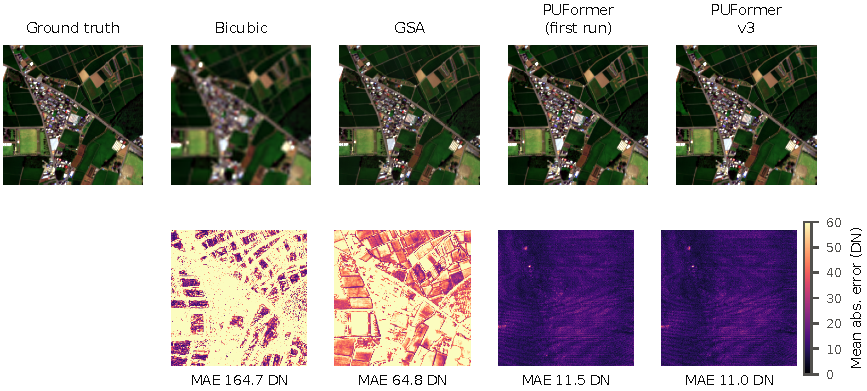
\includegraphics[width=\textwidth]{figures/visual.pdf}
\caption{Test image 7 in false color (bands 60, 40 and 20; top) and the mean absolute error over all bands in DN (bottom; color scale clipped at 60~DN).}
\label{fig:visual}
\end{figure*}

Fig.~\ref{fig:bandwise} shows the error of every band. PUFormer is more accurate than GSA in all 128 bands, and the final model improves on the first run in every band, most at the red edge (700--760~nm), where the mean band RMSE falls from 7.9 to 4.2~DN (from 9.8 to 1.1~DN at 724~nm). The error is largest in the first eight bands (363--404~nm), which lie below the first WorldView-2 band and therefore receive no high-resolution detail from the multispectral image, and in the last bands near 1000~nm, where the sensor's signal-to-noise ratio drops.

\begin{figure*}[t]
\centering
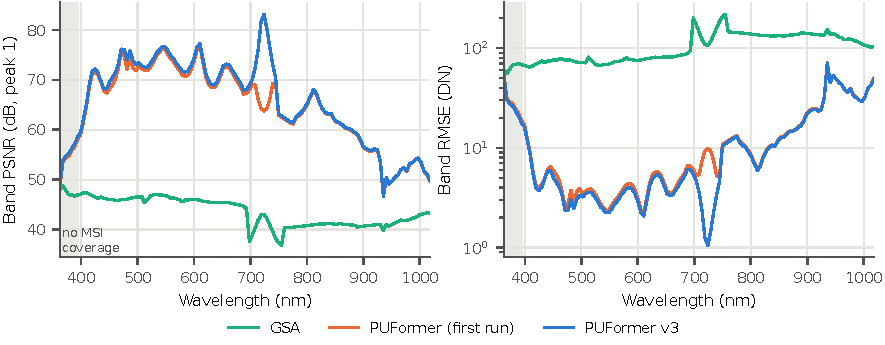
\includegraphics[width=\textwidth]{figures/bandwise.pdf}
\caption{Band-wise PSNR (left, peak 1) and RMSE in DN (right, log scale) over the test set. The shaded range has no multispectral coverage.}
\label{fig:bandwise}
\end{figure*}

\subsection{Training stages and the exact border}
Table~\ref{tab:stages} traces the path from the first run to the final model. Evaluating the first-run weights with the exact reflect-border operator, without retraining, drops the validation PSNR from 58.60 to 49.52~dB. The prior had learned to undo the error that the zero-padded operator introduces at the border, so with the exact operator it over-corrects there; the effect is strongest on the small $64\times64$ validation patches, where border pixels are a large fraction of the image. Fine-tuning removes this within 2000 iterations (58.60~dB validation) and ends at 58.72~dB. The consistency of the reconstruction with its inputs rises from 76.7 to 85.5~dB for the LR-HSI and from 75.0 to 89.0~dB for the HR-MSI. Fig.~\ref{fig:training} shows the validation curves; validation PSNR stops improving after about 44{,}000 fine-tuning iterations, and the test PSNR stays between 58.13 and 58.15~dB from iteration 26{,}000 onward.

\begin{table}[t]
\centering
\caption{From the first run to the final model (test set unless marked). Cons.: $\mathrm{PSNR}(\D\hat{\X},\YH)$ / $\mathrm{PSNR}(\R\hat{\X},\YM)$ in dB}
\label{tab:stages}
\setlength{\tabcolsep}{3pt}
\resizebox{\columnwidth}{!}{%
\begin{tabular}{@{}lccccc@{}}
\toprule
Model & Val. & PSNR & SAM & ERGAS & Cons. \\
\midrule
GSA & -- & 43.20 & 2.730 & 3.279 & 45.4 / 45.0 \\
First run (zero border) & 58.60 & 57.99 & 0.728 & 1.356 & 76.7 / 75.0 \\
\quad + self-ensemble & -- & 58.02 & 0.726 & 1.353 & 76.8 / 75.0 \\
First-run weights, exact border & 49.52 & 54.24 & 0.773 & 1.474 & -- \\
v3 (exact border, full loss) & 58.72 & 58.15 & 0.717 & 1.337 & 85.5 / 89.0 \\
\quad + self-ensemble & -- & 58.20 & 0.713 & 1.330 & 86.0 / 89.5 \\
\bottomrule
\end{tabular}}
\end{table}

\begin{figure*}[t]
\centering
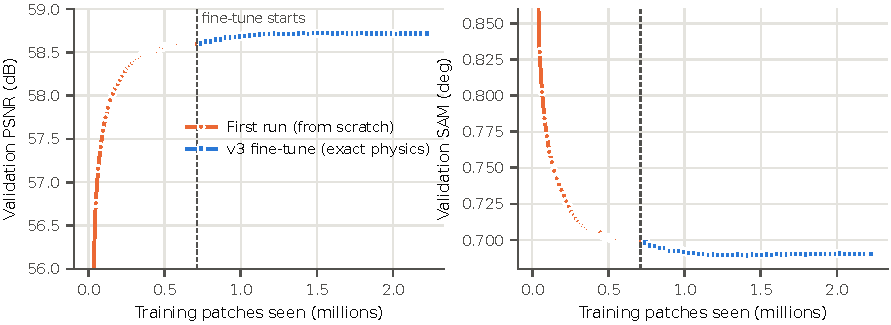
\includegraphics[width=\textwidth]{figures/training.pdf}
\caption{Validation PSNR and SAM during training, plotted against the number of $64\times64$ training patches seen. The first run starts from random weights (its first two evaluations lie below the plotted range); v3 continues from its final weights with the exact border and the full loss.}
\label{fig:training}
\end{figure*}

\subsection{Robustness and test-time operator swap}
Published methods are usually trained and tested with the same degradation. We test the final model on inputs made with a different blur or a shifted spectral response, and with Gaussian noise added to both observations (Table~\ref{tab:robust}, Fig.~\ref{fig:robust}). Because the operators are explicit, PUFormer can also be given the true test-time operator without retraining (``swap''). With the training operator, a blur mismatch costs 3.9--7.5~dB. With the true blur swapped in, the loss is at most 0.26~dB for $\sigma$ between 1.5 and 3.0; with the zero-border operators of the first run, the same swap recovered only to 55.2--57.1~dB. A shifted spectral response is not compensated by the swap, which lowers the PSNR by a further 0.5~dB: the priors, trained with one response, rely on it beyond the data step. Noise is the main weakness of a model trained on noise-free data; PUFormer still exceeds GSA by 10.0~dB at 40~dB SNR and by 2.8~dB at 30~dB SNR.

\begin{table}[t]
\centering
\caption{Robustness of PUFormer v3 (test PSNR in dB / SAM in degrees). Fixed: training operator; swap: true operator supplied at test time}
\label{tab:robust}
\setlength{\tabcolsep}{3pt}
\resizebox{\columnwidth}{!}{%
\begin{tabular}{@{}lccc@{}}
\toprule
Condition & GSA & PUFormer fixed & PUFormer swap \\
\midrule
Nominal & 43.20 / 2.73 & 58.15 / 0.72 & -- \\
Blur $\sigma=1.5$ & 44.05 / 2.57 & 50.68 / 1.15 & \best{57.97 / 0.73} \\
Blur $\sigma=2.5$ & 42.77 / 2.82 & 54.26 / 0.88 & \best{58.05 / 0.72} \\
Blur $\sigma=3.0$ & 42.54 / 2.87 & 51.69 / 1.03 & \best{57.89 / 0.74} \\
SRF shift $-8$~nm & 42.86 / 2.91 & \best{53.01 / 1.20} & 52.54 / 1.31 \\
SRF shift $+8$~nm & 43.29 / 2.68 & \best{53.03 / 1.19} & 52.47 / 1.28 \\
Noise, 40~dB SNR & 43.04 / 2.85 & \best{53.03 / 1.39} & -- \\
Noise, 35~dB SNR & 42.71 / 3.09 & \best{49.11 / 2.20} & -- \\
Noise, 30~dB SNR & 41.84 / 3.67 & \best{44.62 / 3.69} & -- \\
\bottomrule
\end{tabular}}
\end{table}

\begin{figure}[t]
\centering
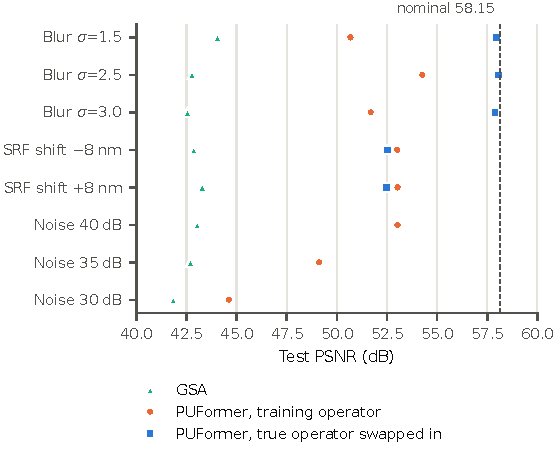
\includegraphics[width=\columnwidth]{figures/robustness.pdf}
\caption{Test PSNR under degradation mismatch and noise. The dashed line is the nominal PUFormer result.}
\label{fig:robust}
\end{figure}

\subsection{Where the Q2n gap comes from}
\label{sec:q2n}
Q2n normalizes every band of every $32\times32$ block by the ground truth's own mean and standard deviation in that block, so an error that is small in absolute terms counts heavily in a band that is nearly flat within a block. Table~\ref{tab:q2n} and Fig.~\ref{fig:q2n} decompose the Q2n of the final model (\QtwonVthree). If the eight ultraviolet bands (363--404~nm) were reconstructed exactly, Q2n would rise to \QtwonExactUV; if the last 24 bands were exact as well, to \QtwonExactUVNIR. In the worst 10\% of blocks, the error energy of these eight bands equals \RelErrUV\ of the ground truth's local variance, against at most \RelErrMaxOther\ for any other group of eight bands. The fine detail of these bands cannot be predicted from the inputs: a least-squares injection of the multispectral detail, fitted on the test ground truth itself, reduces the band-1 error only from \OracleBicA\ to \OracleLinA~DN, while PUFormer reaches \OracleModelA~DN, and PUFormer is more accurate than this oracle in every band we checked.
Q2n is therefore nearly insensitive to overall accuracy on these test images: blending our reconstruction toward bicubic interpolation lowers the PSNR from \CalibPsnrHi\ to \CalibPsnrMid~dB but Q2n only from \CalibQHi\ to \CalibQMid\ (Fig.~\ref{fig:q2n}, right). The values reported in~\cite{chen2026twostage} do not follow PSNR in this way. Between 52.2 and 53.6~dB they range from 0.9832 (DCT) to 0.9963 (DDIF); of the 16 methods within the PSNR range of our curve, 11 lie above it and 5 below. U2Net, for example, is listed at 0.9928 at 50.55~dB, a value our implementation reaches only near 57.6~dB. We conclude that the Q2n values of~\cite{chen2026twostage} were most likely computed with a different implementation, normalization or test region, and that they are not directly comparable with ours.

\begin{table}[t]
\centering
\caption{Q2n analysis of PUFormer v3 (self-ensemble, test set)}
\label{tab:q2n}
\setlength{\tabcolsep}{4pt}
\begin{tabular}{@{}lc@{}}
\toprule
Setting & Q2n \\
\midrule
PUFormer v3 & \QtwonVthree \\
\quad bands 1--8 (363--404~nm) set to ground truth & \QtwonExactUV \\
\quad bands 1--8 and 105--128 set to ground truth & \QtwonExactUVNIR \\
\midrule
Deficit share, worst 10\% / 50\% of blocks & \DefTen\ / \DefFifty \\
\bottomrule
\end{tabular}
\end{table}

\begin{figure*}[t]
\centering
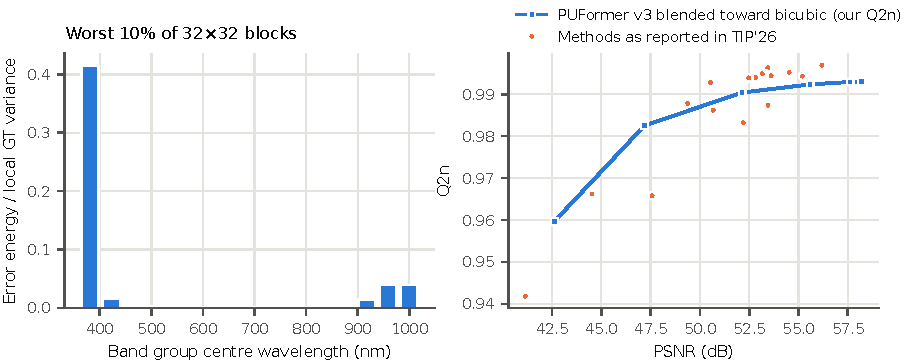
\includegraphics[width=\textwidth]{figures/q2n.pdf}
\caption{Left: error energy relative to the local ground-truth variance per group of eight bands in the worst 10\% of $32\times32$ blocks. Right: Q2n against PSNR when PUFormer's output is blended toward bicubic interpolation (our implementation), and the (PSNR, Q2n) pairs reported in~\cite{chen2026twostage}.}
\label{fig:q2n}
\end{figure*}

\subsection{Complexity}
PUFormer has 10.13~M parameters and needs 18.6~GFLOPs for a $64\times64$ patch and 297~GFLOPs for a $256\times256$ image. On one Tesla T4 it reconstructs a $256\times256$ image with 128 bands in 0.20~s with mixed precision, and the self-ensemble doubles this. Because the attention is computed across channels, memory and time grow linearly with the number of pixels.

\section{Discussion and Limitations}
Three caveats apply to the comparison. First, our test images follow the protocol as described in~\cite{chen2026twostage}, but they may not be the exact pixels used there, and all other rows of Table~\ref{tab:main} are reported values. RMSE in digital numbers, which does not depend on a peak or data range, is the most robust basis for comparison, and there PUFormer's lead (18.9 vs.\ 25.7~DN) is largest. Second, SSIM depends strongly on its data range: with the stricter per-image range, PUFormer's SSIM (0.9970) is below the value reported in~\cite{chen2026twostage}. Third, as shown above, Q2n on these images is dominated by bands that no method can reconstruct well. Beyond the comparison, the model is trained without noise and for one sensor pair; the swap experiment shows that the exact operators make the network adaptable to the blur but not to the spectral response, and training with noise and with randomized responses is a natural next step. Evaluation on further datasets is left for future work.

\section{Conclusion}
PUFormer combines exact data-consistency steps, including the correct image border and its adjoint, with a transposed-attention prior and cross-stage memory. Under a fully specified Chikusei $\times$4 protocol it improves on the best reported result by 2.0~dB PSNR and 26\% RMSE and ranks first on seven of eight metrics, while its reconstructions reproduce both observations to within 86--90~dB. The exact operators also let the model absorb a blur mismatch at test time with almost no loss. All code, training logs, result files and the evaluation scripts, including the metric implementations, are publicly available.

\section*{Acknowledgment}
The author thanks N. Yokoya and A. Iwasaki for making the Chikusei data available, and Kaggle for the GPU time used to train and evaluate the models.

\bibliographystyle{IEEEtran}
\bibliography{references}

\end{document}
